\documentclass[11pt, a4paper]{article}\usepackage[]{graphicx}\usepackage[]{color}
%% maxwidth is the original width if it is less than linewidth
%% otherwise use linewidth (to make sure the graphics do not exceed the margin)
\makeatletter
\def\maxwidth{ %
  \ifdim\Gin@nat@width>\linewidth
    \linewidth
  \else
    \Gin@nat@width
  \fi
}
\makeatother

\definecolor{fgcolor}{rgb}{0.345, 0.345, 0.345}
\newcommand{\hlnum}[1]{\textcolor[rgb]{0.686,0.059,0.569}{#1}}%
\newcommand{\hlstr}[1]{\textcolor[rgb]{0.192,0.494,0.8}{#1}}%
\newcommand{\hlcom}[1]{\textcolor[rgb]{0.678,0.584,0.686}{\textit{#1}}}%
\newcommand{\hlopt}[1]{\textcolor[rgb]{0,0,0}{#1}}%
\newcommand{\hlstd}[1]{\textcolor[rgb]{0.345,0.345,0.345}{#1}}%
\newcommand{\hlkwa}[1]{\textcolor[rgb]{0.161,0.373,0.58}{\textbf{#1}}}%
\newcommand{\hlkwb}[1]{\textcolor[rgb]{0.69,0.353,0.396}{#1}}%
\newcommand{\hlkwc}[1]{\textcolor[rgb]{0.333,0.667,0.333}{#1}}%
\newcommand{\hlkwd}[1]{\textcolor[rgb]{0.737,0.353,0.396}{\textbf{#1}}}%
\let\hlipl\hlkwb

\usepackage{framed}
\makeatletter
\newenvironment{kframe}{%
 \def\at@end@of@kframe{}%
 \ifinner\ifhmode%
  \def\at@end@of@kframe{\end{minipage}}%
  \begin{minipage}{\columnwidth}%
 \fi\fi%
 \def\FrameCommand##1{\hskip\@totalleftmargin \hskip-\fboxsep
 \colorbox{shadecolor}{##1}\hskip-\fboxsep
     % There is no \\@totalrightmargin, so:
     \hskip-\linewidth \hskip-\@totalleftmargin \hskip\columnwidth}%
 \MakeFramed {\advance\hsize-\width
   \@totalleftmargin\z@ \linewidth\hsize
   \@setminipage}}%
 {\par\unskip\endMakeFramed%
 \at@end@of@kframe}
\makeatother

\definecolor{shadecolor}{rgb}{.97, .97, .97}
\definecolor{messagecolor}{rgb}{0, 0, 0}
\definecolor{warningcolor}{rgb}{1, 0, 1}
\definecolor{errorcolor}{rgb}{1, 0, 0}
\newenvironment{knitrout}{}{} % an empty environment to be redefined in TeX

\usepackage{alltt}
\usepackage[margin=1in]{geometry}
\usepackage[utf8]{inputenc}
\usepackage[english]{babel}
\usepackage{csquotes}
\usepackage{longtable, booktabs, tabularx, threeparttable, adjustbox}
\usepackage{amsmath, amssymb, amsthm, bbm, bm}
\usepackage{secdot, sectsty}
\usepackage{hyperref}
\usepackage{pdflscape}
\usepackage{geometry}
\usepackage{placeins}
\usepackage{caption}
\usepackage{graphicx}
\usepackage{setspace}

\usepackage[backend=bibtex, style=authortitle, citestyle=authoryear-icomp, url=false]{biblatex}
\addbibresource{UBIF.bib}

\AtBeginEnvironment{quote}{\singlespacing\small}

\allsectionsfont{\rmfamily}
\sectionfont{\normalsize}
\subsectionfont{\normalfont\normalsize\selectfont\itshape}
\subsubsectionfont{\normalfont\normalsize\selectfont\itshape}

\newcommand{\specialcell}[2][c]{%
      \begin{tabular}[#1]{@{}c@{}}#2\end{tabular}}
\IfFileExists{upquote.sty}{\usepackage{upquote}}{}
\begin{document}

\title{\textsc{Framing an Unconditional Cash Transfer: Pre-Analysis Plan}}
\author{Author\footnote{The Busara Center for Behavioral Economics}}

\maketitle

\begin{abstract}

    This document describes the pre-analysis plan for a randomized experiment examining the effects of framing of welfare payments on self-concept and economic behavior. In this study, we will provide small, unconditional cash transfers to residents of an informal settlement in Nairobi and vary the way in which the transfers are framed to participants. Participants will be randomly assigned to one of three treatment groups: the transfer framed as a means toward poverty alleviation, individual empowerment, or collective support. We will then collect self-reported measures of self-efficacy, judgement, and affect and observed measures of temporal discounting and investment. This pre-analysis plan outlines our hypotheses, the schedule of experimental tasks, and our empirical strategy. In order to guarantee transparency and bind ourselves from fishing for results, we will pre-register the source files to be used for data analysis.

\end{abstract}

\newpage

\tableofcontents

\newpage

\section{Introduction}

\section{Research Design}

    \subsection{Sampling}

        This study will be conducted in conjunction with the Busara Center for Behavioral Economics in Nairobi with 525 participants residing in Kibera, one of Kenya's largest urban slums \parencite{haushofer_methodology_2014}. Treatment and data collection will take place with household surveys in the Kibera settlement with Busara Center enumerators. This section outlines the sampling procedure to be used in the experiment.

        The study area will be partitioned into non-overlapping catchment regions to be used for sample selection. Research staff will visit one catchment region per day and will not visit the same region more than once. Beginning at a designated intersection in the catchment region, a team of nine enumerators and a guide\footnote{Guides will accompany enumerators but will not be involved in sampling or data collection.} will select every eighth household in each direction for survey. From that visit on, enumerators will select the eighth house down from the subsequent structure, away from the intersection and on the opposite side of the road. If participants are not available at the selected households enumerators will move to the next door away from the origin.

        Sampled individuals will be enrolled in the survey if they meet the following eligibility criteria:

        \begin{enumerate}
            \item Between 18 and 50 years old
            \item Resident of Kibera
            \item Not surveyed by the Busara Center for any other study in the past 10 days
            \item Owns a working phone with Safaricom
        \end{enumerate}

        If an eligible person is available at the selected household, they will be enrolled as a participant. If there are multiple members, enumerators will prioritize the youngest eligible person of the opposite gender than in the previous survey. We will sample from the study area for a total of 525 surveys.

        % Check that this is updated
        % What is the extent of the study area in Kibera?
        % How do we define catchment areas (regions)?

    \subsection{Statistical power}

        % Include any power calculations here

    \subsection{Experimental procedure}

        The survey questionnaire will be delivered in English with Kiswahili translations. The following summarizes the schedule of tasks in the questionnaire.\footnote{We will use a single survey instrument, programmed with Qualtrics, for treatment delivery and subsequent data collection. The programmed and paper versions of the survey are included as supplementary materials.}

        \begin{enumerate}
            \item Consent agreement
            \item Cash transfer framing
            \item Self-efficacy questionnaire (5 items)
            \item Judgement questionnaire (5 items)
            \item Affect questionnaire (4 items)
            \item Video selection task
            \item Savings task
            \item Frame evaluation
            \item Message of support
            \item Subjective social status ladder scale (2 items)
            \item Sociodemographic questionnaire (9 items)
        \end{enumerate}

    \subsection{Treatment}

        At the outset of the survey, eligible and consenting participants will be told they are receiving an unconditional cash transfer of KES 400 (USD PPP 10.5) from an organization unaffiliated with the Busara Center.\footnote{This study will be conducted with Kenyan shillings (KES). We report USD values calculated at purchasing power parity using a conversion factor for private consumption of 38.15 in 2013. The price level ratio of PPP conversion factor (GDP) to KES market exchange rate for 2011 was 0.444.} Participants will be randomly assigned by the survey software\footnote{We evenly assign treatment groups to achive balance in group size.} to receive one of three messages introducing the purpose of the cash transfer. All frames are identical in content and structure save for the described purpose of the cash transfer. In the poverty allevation framing, the payment is described as a means to meet basic needs. The individual empowerment framing describes the payment as a means toward individual goals and the collective support framing as a means toward goals regarding family and the community. Participants will listen to the message in their preferred language (English or Kiswahili) with pre-recorded audio clips or as read by the enumerator.

        After framing, enumerators will send USD PPP 10.5 to the participant via the mobile money system M-Pesa.\footnote{For more information on M-Pesa, we refer the reader to \textcite{jack_mobile_2011} and \textcite{mbiti_mobile_2011}.} Enumerators will be instructed to confirm receipt of the payment. In the individual empowerment and collective support treatments, enumerators will also elicit participants to list either individual or collective goals and beliefs about the purpose of the payment.

        \subsubsection{Poverty alleviation framing}

            \begin{quote}

                The goal of this Poverty Alleviation Organization is to alleviate poverty and reduce financial hardship among the poor. This organization believes that people living in poverty should be given income support to help them meet their basic needs. This organization aims to help promote a decent standard of living among the poor and help them deal with emergencies. Thus, the Poverty Alleviation Organization gives financial assistance to people like you, to help them make ends meet. For example, with the financial assistance, people might be able to struggle less to afford basic needs, like paying off debts, paying rent, and buying clothes and food. Now we are going to send you 400 KSh. Please note that this is a one-time transfer of financial assistance.

            \end{quote}

        \subsubsection{Individual empowerment framing}

            \begin{quote}

                The goal of this Individual Empowerment Organization is to promote individuals' potential to create a better future for themselves.  The organization believes that individuals are wise and know best how to help themselves become self-reliant/independent if they have the financial resources to do so. This organization aims to empower individuals to pursue their personal interests and create their own path to independence. Thus, the Individual Empowerment Organization gives financial resources to individuals, like you, to enable them to invest in their personal goals. For example, people might use their unique talents to start a self-run business, invest in job training courses, or create art. Now we are going to send you 400 KSh. Please note that this is a one-time transfer of financial resources.

            \end{quote}

        \subsubsection{Collective support framing}

            \begin{quote}

                The goal of this Community Empowerment Organization is to enable people to help promote better futures for those they care about and want to support most. The organization believes that people know best how to support each other and grow together if they have financial resources to do so. This organization aims to empower people to improve their own lives and those of the people and communities they care about most. Thus, the Community Empowerment Organization gives financial resources to community members, like you, to enable them to contribute positively to the lives of people important to them. For example, when people can invest in themselves, they are better able to expand employment opportunities for others, provide valuable services to their community, or teach others, including children, useful skills and knowledge. Now Community Empowerment Organization is going to send you 400 KSh. Please note that this is a one-time transfer of financial resources.

            \end{quote}

\section{Data}

    \subsection{Cash transfer framing}
    \subsection{Self-efficacy questionnaire (5 items)}
    \subsection{Judgement questionnaire (5 items)}
    \subsection{Affect questionnaire (4 items)}
    \subsection{Video selection task}
    \subsection{Savings task}
    \subsection{Frame evaluation}
    \subsection{Message of support}
    \subsection{Subjective social status ladder scale (2 items)}
    \subsection{Sociodemographic questionnaire (9 items)}

\section{Empirical Analysis}

    \subsection{Treatment effect of cash transfer frames}

        % Specify balance checks?

        We will use the following reduced-form specification to estimate the treatment effect of different frames.\footnote{We will conduct the data analysis outlined in this section using the R programming language with the scripts included in Appendix \ref{sec:rscripts}.}

  		\begin{equation} \label{eq:teffect}
            Y_{i} = \beta_{0} + \beta_{1}\text{\textsc{Ind}}_{i} + \beta_{2}\text{\textsc{Com}}_{i} + \varepsilon_{i}
		\end{equation}

        $Y_{i}$ refers to the outcome variables for individual $i$ measured after the manipulation. The outcome variables described in Table \ref{tab:depvars} will be the focus of this analysis. \textsc{Ind}$_{i}$ indicates assignment to the individual empowerment frame while \textsc{Com}$_{i}$ indicates assignment to the collective support frame. The reference category in this model is the poverty alleviation frame. We will estimate cluster-robust standard errors at the individual level. Table \ref{tab:hypotheses} lists the hypotheses we will test using Equation \ref{eq:teffect}.

        % Separately specify mechanism analysis?

        \begin{table}[h]
        \centering
        \caption{Primary outcome variables}
        \label{tab:depvars}
        \maxsizebox*{\textwidth}{\textheight}{
        \begin{tabular}{@{}lllll@{}}
        \toprule
        Variable & Description &  &  &  \\ \midrule
        Video selection & Dummy variable for having chosen at least one business video &  &  &  \\
        Savings choice & Dummy variable for sending non-zero amount &  &  &  \\
        Message recording & Dummy variable for recording message of support &  &  &  \\
        Effect forecast & &  &  &  \\
        \bottomrule
        \end{tabular} }
        \end{table}

        \begin{table}[h]
        \centering
        \caption{Primary hypothesis tests}
        \label{tab:hypotheses}
        \maxsizebox*{\textwidth}{\textheight}{
        \begin{tabular}{@{}lllll@{}}
        \toprule
        Null hypothesis & Description &  &  &  \\ \midrule
        $H_0: \beta_1 = 0$ & Effect of individual empowerment frame relative to poverty alleviation frame &  &  &  \\
        $H_0: \beta_2 = 0$ & Effect of collective support frame relative to poverty alleviation frame &  &  &  \\
        $H_0: \beta_1 = \beta_2$ & Effect of collective support frame relative to individual empowerment frame &  &  &  \\ \bottomrule
        \end{tabular} }
        \end{table}

        To improve precision, we will also apply covariate adjustment with a vector of baseline indicators $\mathbf{X}_i$. We obtain the covariate-adjusted treatment effect estimate by estimating Equation \ref{eq:teffect} including the demeaned covariate vector $\mathbf{\dot X}_{i} = \mathbf{X}_{i} - \mathbf{\bar X}_{i}$ as an additive term and as an interaction with the treatment indicator. % scrap this maybe

        \begin{equation} \label{eq:controls}
            Y_{i} = \beta_{0} + \beta_{1}\text{\textsc{Ind}}_{i} + \beta_{2}\text{\textsc{Com}}_{i} + \gamma_{0} \mathbf{\dot X}'_i + \gamma_{1}\text{\textsc{Ind}}_{i} \mathbf{\dot X}'_i + \gamma_{2}\text{\textsc{Com}}_{i} \mathbf{\dot X}'_i + \varepsilon_{i}
        \end{equation}

        The set of indicators partitions our sample so that our estimate for $\beta_j$ remains unbiased for the average treatment effect \parencite{lin_agnostic_2013}. We will estimate cluster-robust standard errors at the individual level. We use this model to test the hypotheses detailed in Table \ref{tab:hypotheses} including the control variables listed in Table \ref{tab:controlvars}.

        \begin{table}[h]
        \centering
        \caption{Control variables for covariate adjustment}
        \label{tab:controlvars}
        \maxsizebox*{\textwidth}{\textheight}{
        \begin{tabular}{@{}lllll@{}}
        \toprule
        Variable & Description &  &  &  \\ \midrule
        Age & Dummy variable indicating participant is over 25 &  &  &  \\
        Gender & Dummy variable indicating participant is female &  &  &  \\
        Employment & Dummy variable indicating participant is employed &  &  &  \\
        Education & Dummy variable indicating participant completed std. 8 &  &  &  \\
        Savings & Dummy variable having more than Ksh 1000 saved &  &  &  \\
        \bottomrule
        \end{tabular} }
        \end{table}

    \subsection{Randomization inference} % scrap this maybe

        One potential concern is that inference might be invalidated by finite sample bias in estimates of the standard errors. To address this issue, we will conduct randomization inference to test the Fisherian sharp null hypothesis of no treatment effect for every participant \parencite{fisher_design_1935}.\footnote{Note that this is more restrictive than the null hypothesis of zero average treatment effect we will test in the previous section.} We perform Monte Carlo approximations of the exact $p$-values using $M=10,000$ permutations of the treatment assignment. We will then estimate our primary specification within each $m^{th}$ permutation and calculate the standard Wald statistics for each of our hypothesis tests. We will compare the Wald statistics from the original sample with the distribution of permuted statistics to produce approximations of the exact $p$-values:

        \begin{equation} \label{eq:exactp}
            \hat{p}_{\beta} =  \frac{1}{10,000}\sum_{m=1}^{10,000} \mathbf{1} \Big [ \mathbf{\hat{\beta'}}_m V(\mathbf{\hat{\beta}}_m)^{-1} \mathbf{\hat{\beta}}_m \geq \mathbf{\hat{\beta'}}_{obs.} V(\mathbf{\hat{\beta}}_{obs.})^{-1} \hat{\beta}_{obs.} \Big ]
        \end{equation}

        Following \textcite{young_channeling_2015}, we will permute the data and calculate the regressions for all outcomes within each draw.

    \subsection{Multiple testing adjustment}

        Given that our survey instrument included several items related to a single behavior or dimension, we will calculate sharpened $q$-values over outcomes in Table \ref{tab:depvars} to control the false discovery rate \parencite{benjamini_adaptive_2006}. Rather than specifying a single $q$, we will report the minimum $q$-value at which each hypothesis is rejected \parencite{anderson_multiple_2008}. We will apply this correction separately for each hypothesis test and will report both standard $p$-values and minimum $q$-values in our analysis.

    \subsection{Heterogeneous treatment effects}

        We will analyze the extent to which the policy frames produced heterogeneous treatment effects with the following specification.

        \begin{equation}
            Y_{i} = \beta_{0} + \beta_{1}\text{\textsc{Ind}}_{i} + \beta_{2}\text{\textsc{Com}}_{i} + \delta_{0} x_i + \delta_{1}\text{\textsc{Ind}}_{i} x_i + \delta_{2}\text{\textsc{Com}}_{i} x_i + \varepsilon_{i}
        \label{eq:heteffect} \end{equation}

        $x_{i}$ is the binary dimension of heterogeneity measured before treatment assignment. $\delta_{1}$ and $\delta_{2}$ identify the heterogeneous treatment effects of the individual empowerment and collective support frames relative to the poverty alleviation frame. Testing $\delta_{1} = \delta_{2}$ identifies heterogeneous effects between the former two frames. Standard errors are clustered at the individual level. We estimate this model with the baseline variables summarized in Table \ref{tab:controlvars}.

    \subsection{Analysis of potential mechanisms}

\newpage

\printbibliography

\newpage

\appendix

\section{Consent Form}

    \maxsizebox*{\textwidth}{\textheight}{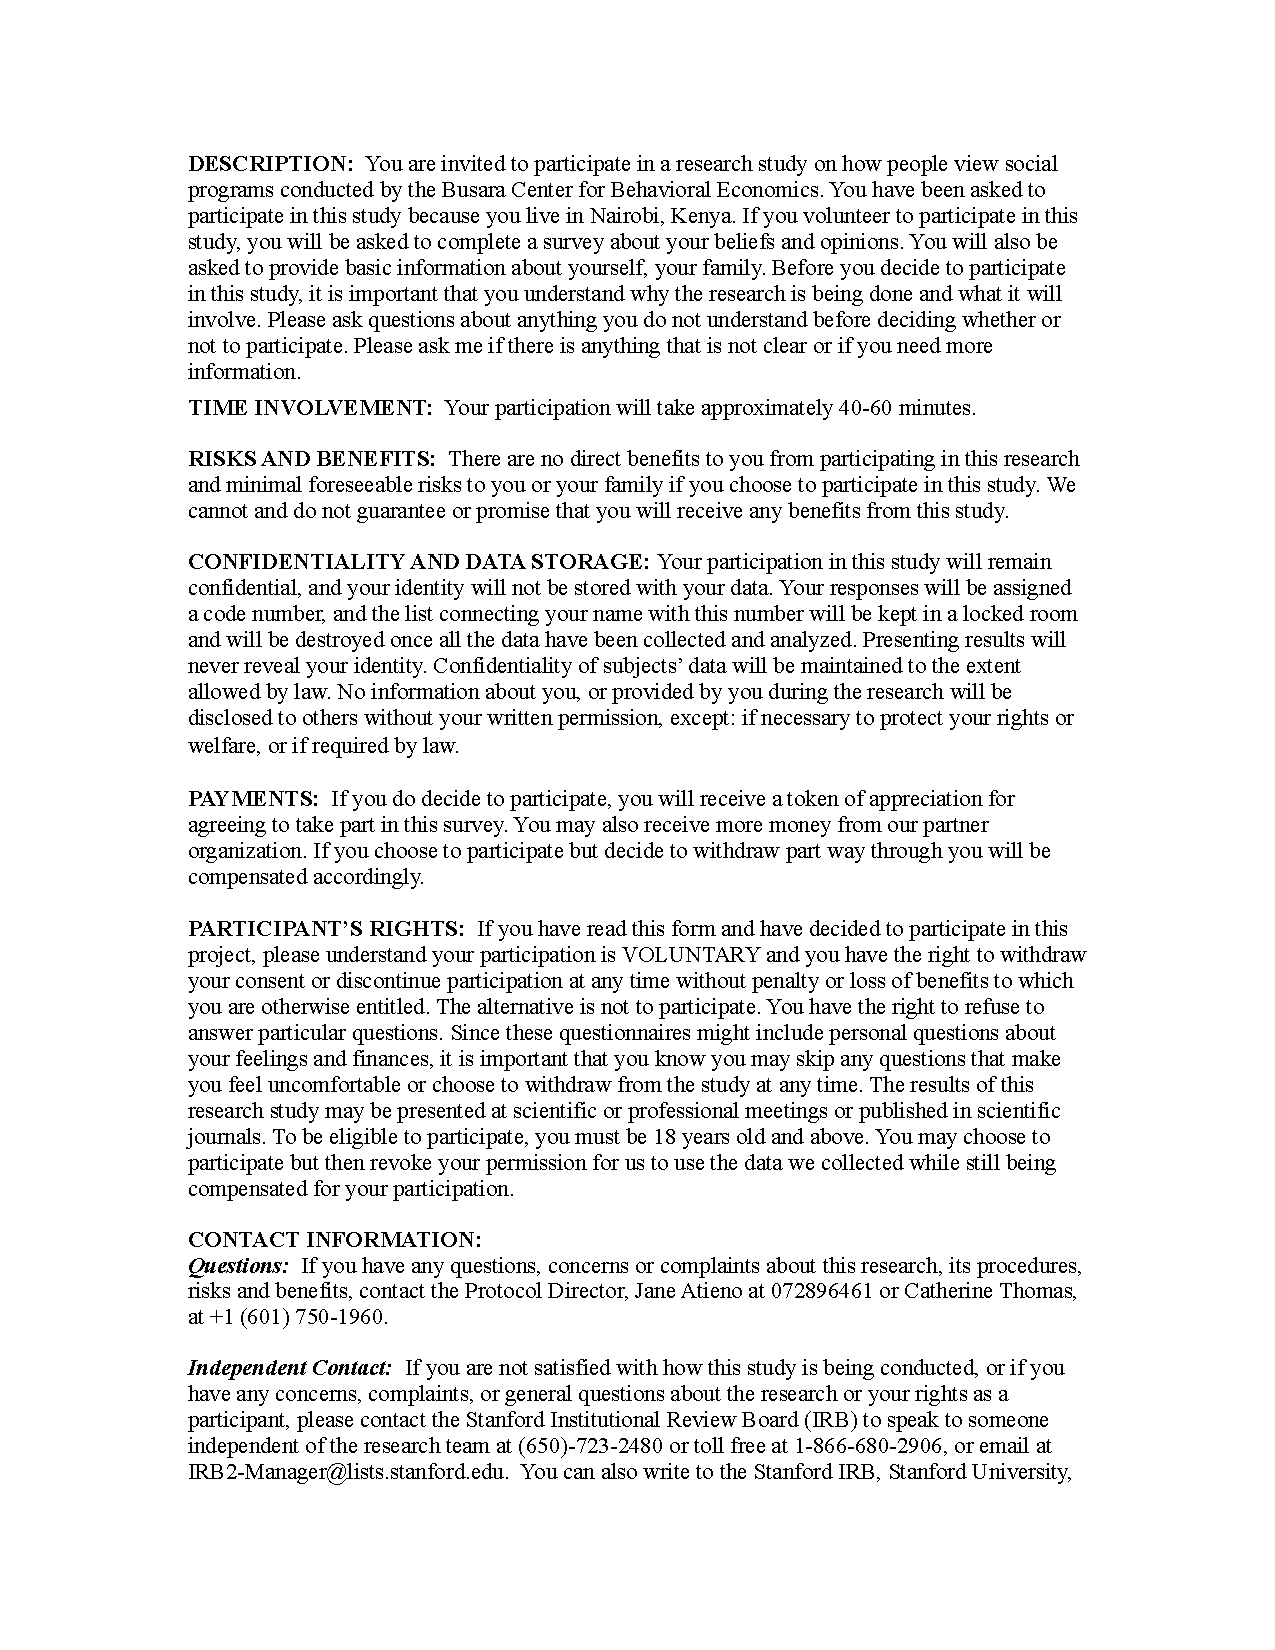
\includegraphics[page=1]{UBI_Consent_S4_Kenya.pdf}}
    \maxsizebox*{\textwidth}{\textheight}{\includegraphics[page=2]{UBI_Consent_S4_Kenya.pdf}}
    \maxsizebox*{\textwidth}{\textheight}{\includegraphics[page=3]{UBI_Consent_S4_Kenya.pdf}}

\section{Survey Instrument}

\section{Data Analysis Scripts} \label{sec:rscripts}

    \subsection{Packages}

\begin{knitrout}
\definecolor{shadecolor}{rgb}{0.969, 0.969, 0.969}\color{fgcolor}\begin{kframe}
\begin{alltt}
    \hlkwd{setwd}\hlstd{(}\hlstr{"/Users/Justin/Google Drive/UBIF/UBIF_Deliverables/UBIF_PAP/K1_PAP"}\hlstd{)} \hlcom{# make this more flexible}
    \hlkwd{set.seed}\hlstd{(}\hlnum{47269801}\hlstd{)}

    \hlstd{required.packages} \hlkwb{<-} \hlkwd{c}\hlstd{(}\hlstr{"dplyr"}\hlstd{,} \hlstr{"multiwayvcov"}\hlstd{,} \hlstr{"multcomp"}\hlstd{,} \hlstr{"knitr"}\hlstd{)}
    \hlstd{packages.missing} \hlkwb{<-} \hlstd{required.packages[}\hlopt{!}\hlstd{required.packages} \hlopt \hlkwd{installed.packages}\hlstd{()[,}\hlstr{"Package"}\hlstd{]]}

    \hlkwa{if}\hlstd{(}\hlkwd{length}\hlstd{(packages.missing)} \hlopt{>} \hlnum{0}\hlstd{) \{}\hlkwd{install.packages}\hlstd{(required.packages,} \hlkwc{repo}\hlstd{=}\hlstr{"https://cran.cnr.berkeley.edu/"}\hlstd{)\}}
    \hlkwd{lapply}\hlstd{(required.packages, library,} \hlkwc{character.only} \hlstd{=} \hlnum{TRUE}\hlstd{)}
\end{alltt}
\end{kframe}
\end{knitrout}

    \subsection{User-defined functions}

\begin{knitrout}
\definecolor{shadecolor}{rgb}{0.969, 0.969, 0.969}\color{fgcolor}\begin{kframe}
\begin{alltt}
    \hlcom{## RegTest conducts asymptotic test from linear model ##}

    \hlstd{RegTest} \hlkwb{<-} \hlkwa{function}\hlstd{(}\hlkwc{equation}\hlstd{,} \hlkwc{clustvars}\hlstd{,} \hlkwc{hypotheses}\hlstd{,} \hlkwc{data}\hlstd{) \{}

        \hlstd{model} \hlkwb{<-} \hlkwd{lm}\hlstd{(equation,} \hlkwc{data} \hlstd{= data,} \hlkwc{na.action} \hlstd{= na.omit)}

        \hlkwa{if} \hlstd{(}\hlkwd{missing}\hlstd{(clustvars)) model}\hlopt{$}\hlstd{vcov} \hlkwb{<-} \hlkwd{vcov}\hlstd{(model)}
        \hlkwa{else} \hlstd{model}\hlopt{$}\hlstd{vcov} \hlkwb{<-} \hlkwd{cluster.vcov}\hlstd{(model,} \hlkwc{cluster} \hlstd{= clustvars)}

        \hlstd{model}\hlopt{$}\hlstd{test} \hlkwb{<-} \hlkwd{summary}\hlstd{(}\hlkwd{glht}\hlstd{(model,} \hlkwc{linfct} \hlstd{= hypotheses,} \hlkwc{vcov} \hlstd{= model}\hlopt{$}\hlstd{vcov))}\hlopt{$}\hlstd{test}

        \hlstd{numhyp} \hlkwb{<-} \hlkwd{length}\hlstd{(hypotheses)}

        \hlstd{EST} \hlkwb{<-} \hlkwd{matrix}\hlstd{(}\hlkwc{nrow} \hlstd{= numhyp,} \hlkwc{ncol} \hlstd{=} \hlnum{4}\hlstd{)}

        \hlkwa{for} \hlstd{(i} \hlkwa{in} \hlnum{1}\hlopt{:}\hlstd{numhyp) \{}

            \hlstd{EST[i,} \hlnum{1}\hlstd{]} \hlkwb{<-} \hlstd{model}\hlopt{$}\hlstd{test}\hlopt{$}\hlstd{coefficients[i]}
            \hlstd{EST[i,} \hlnum{2}\hlstd{]} \hlkwb{<-} \hlstd{model}\hlopt{$}\hlstd{test}\hlopt{$}\hlstd{tstat[i]}
            \hlstd{EST[i,} \hlnum{3}\hlstd{]} \hlkwb{<-} \hlstd{model}\hlopt{$}\hlstd{test}\hlopt{$}\hlstd{sigma[i]}
            \hlstd{EST[i,} \hlnum{4}\hlstd{]} \hlkwb{<-} \hlstd{model}\hlopt{$}\hlstd{test}\hlopt{$}\hlstd{pvalues[i]}

        \hlstd{\}}

        \hlkwd{colnames}\hlstd{(EST)} \hlkwb{<-} \hlkwd{c}\hlstd{(}\hlstr{"Estimate"}\hlstd{,} \hlstr{"Tstat"}\hlstd{,} \hlstr{"SE"}\hlstd{,} \hlstr{"P"}\hlstd{)}

        \hlkwd{return}\hlstd{(EST)}

    \hlstd{\}}

    \hlcom{## PermTest returns MC approximations of the exact p-value ##}

    \hlstd{PermTest} \hlkwb{<-} \hlkwa{function}\hlstd{(}\hlkwc{equation}\hlstd{,} \hlkwc{treatvars}\hlstd{,} \hlkwc{clustvars}\hlstd{,} \hlkwc{hypotheses}\hlstd{,} \hlkwc{iterations}\hlstd{,} \hlkwc{data}\hlstd{) \{}

        \hlkwd{stopifnot}\hlstd{(}\hlkwd{length}\hlstd{(hypotheses)} \hlopt{<=} \hlnum{1}\hlstd{)}

        \hlstd{obsEST} \hlkwb{<-} \hlkwd{RegTest}\hlstd{(equation, clustvars, hypotheses, data)}
        \hlstd{obsStat} \hlkwb{<-} \hlstd{obsEST[}\hlnum{1}\hlstd{,} \hlnum{2}\hlstd{]}

        \hlstd{simEST} \hlkwb{<-} \hlkwd{matrix}\hlstd{(}\hlkwc{ncol} \hlstd{=} \hlnum{4}\hlstd{)}

        \hlkwa{for} \hlstd{(i} \hlkwa{in} \hlnum{1}\hlopt{:}\hlstd{iterations) \{}

            \hlstd{simTreat} \hlkwb{<-} \hlstd{data[, treatvars,} \hlkwc{drop} \hlstd{=} \hlnum{FALSE}\hlstd{]}
            \hlstd{simTreat} \hlkwb{<-} \hlstd{simTreat[}\hlkwd{sample}\hlstd{(}\hlkwd{nrow}\hlstd{(simTreat)),]}

            \hlstd{simData} \hlkwb{<-} \hlkwd{cbind}\hlstd{(simTreat, data[,} \hlopt{!}\hlstd{(}\hlkwd{names}\hlstd{(data)} \hlopt \hlstd{treatvars),} \hlkwc{drop} \hlstd{=} \hlnum{FALSE}\hlstd{])}
            \hlkwd{colnames}\hlstd{(simData)[}\hlnum{1}\hlopt{:}\hlnum{2}\hlstd{]} \hlkwb{<-} \hlstd{treatvars}

            \hlstd{simEST} \hlkwb{<-} \hlkwd{rbind}\hlstd{(simEST,} \hlkwd{RegTest}\hlstd{(equation, clustvars, hypotheses,} \hlkwc{data} \hlstd{= simData))}

        \hlstd{\}}

        \hlstd{simSTAT} \hlkwb{<-} \hlstd{simEST[}\hlnum{2}\hlopt{:}\hlkwd{nrow}\hlstd{(simEST),} \hlnum{2}\hlstd{]}
        \hlstd{countSTAT} \hlkwb{<-} \hlkwd{matrix}\hlstd{(}\hlkwd{abs}\hlstd{(simSTAT)} \hlopt{>=} \hlkwd{abs}\hlstd{(obsStat),} \hlkwc{ncol} \hlstd{=} \hlnum{1}\hlstd{)}

        \hlstd{ExactP} \hlkwb{<-} \hlkwd{matrix}\hlstd{(}\hlnum{1}\hlstd{,} \hlkwc{nrow} \hlstd{=} \hlnum{1}\hlstd{,} \hlkwc{ncol} \hlstd{=} \hlkwd{nrow}\hlstd{(countSTAT))} \hlopt \hlstd{countSTAT}
        \hlstd{ExactP} \hlkwb{<-} \hlstd{ExactP} \hlopt{/} \hlstd{iterations}

        \hlstd{EST} \hlkwb{<-} \hlkwd{cbind}\hlstd{(obsEST, ExactP)}

        \hlkwd{colnames}\hlstd{(EST)} \hlkwb{<-} \hlkwd{c}\hlstd{(}\hlstr{"Estimate"}\hlstd{,} \hlstr{"Tstat"}\hlstd{,} \hlstr{"SE"}\hlstd{,} \hlstr{"P"}\hlstd{,} \hlstr{"ExactP"}\hlstd{)}

        \hlkwd{return}\hlstd{(EST)}

    \hlstd{\}}

    \hlcom{## FDR returns minimum q-values ##}

    \hlstd{FDR} \hlkwb{<-} \hlkwa{function}\hlstd{(}\hlkwc{pvals}\hlstd{,} \hlkwc{step}\hlstd{) \{}

        \hlkwa{if} \hlstd{(}\hlkwd{sum}\hlstd{(}\hlkwd{is.na}\hlstd{(pvals)} \hlopt{==} \hlnum{FALSE}\hlstd{)} \hlopt{<=} \hlnum{1}\hlstd{) \{}\hlkwd{return}\hlstd{(pvals)\}}
        \hlkwa{if} \hlstd{(}\hlkwd{missing}\hlstd{(step)) \{step} \hlkwb{<-} \hlnum{0.001}\hlstd{\}}

        \hlstd{allpvals} \hlkwb{<-} \hlkwd{cbind}\hlstd{(}\hlkwd{as.matrix}\hlstd{(pvals),} \hlkwd{matrix}\hlstd{(}\hlnum{1}\hlopt{:}\hlkwd{nrow}\hlstd{(}\hlkwd{as.matrix}\hlstd{(pvals)),} \hlkwc{ncol} \hlstd{=} \hlnum{1}\hlstd{))}

        \hlstd{pvals} \hlkwb{<-} \hlkwd{na.omit}\hlstd{(allpvals)}
        \hlstd{nump} \hlkwb{<-} \hlkwd{nrow}\hlstd{(pvals)}

        \hlstd{pvals} \hlkwb{<-} \hlstd{pvals[}\hlkwd{order}\hlstd{(pvals[,} \hlnum{1}\hlstd{]), ]}
        \hlstd{rank} \hlkwb{<-} \hlkwd{matrix}\hlstd{(}\hlnum{1}\hlopt{:}\hlstd{nump,} \hlkwc{ncol} \hlstd{=} \hlnum{1}\hlstd{)}
        \hlstd{pvals} \hlkwb{<-} \hlkwd{cbind}\hlstd{(pvals, rank,} \hlkwd{matrix}\hlstd{(}\hlnum{0}\hlstd{,} \hlkwc{nrow} \hlstd{= nump,} \hlkwc{ncol} \hlstd{=} \hlnum{1}\hlstd{))}

        \hlstd{qval} \hlkwb{<-} \hlnum{1}

        \hlkwa{while} \hlstd{(qval} \hlopt{>} \hlnum{0}\hlstd{) \{}

            \hlstd{qfirst} \hlkwb{<-} \hlstd{qval} \hlopt{/} \hlstd{(}\hlnum{1} \hlopt{+} \hlstd{qval)}
            \hlstd{fdrtemp} \hlkwb{<-} \hlstd{(qfirst} \hlopt{*} \hlstd{rank)} \hlopt{/} \hlstd{nump}

            \hlstd{subrank} \hlkwb{<-} \hlkwd{which}\hlstd{(fdrtemp} \hlopt{>=} \hlkwd{as.matrix}\hlstd{(pvals[,} \hlnum{1}\hlstd{]))}

            \hlkwa{if} \hlstd{(}\hlkwd{length}\hlstd{(subrank)} \hlopt{<} \hlnum{1}\hlstd{) \{}
                \hlstd{numreject} \hlkwb{<-} \hlnum{0}
            \hlstd{\}} \hlkwa{else} \hlstd{numreject} \hlkwb{<-} \hlkwd{max}\hlstd{(subrank)}

            \hlstd{qsec} \hlkwb{<-} \hlstd{qfirst} \hlopt{*} \hlstd{(nump} \hlopt{/} \hlstd{(nump} \hlopt{-} \hlstd{numreject))}
            \hlstd{fdrtemp} \hlkwb{<-} \hlstd{(qsec} \hlopt{*} \hlstd{rank)} \hlopt{/} \hlstd{nump}

            \hlstd{subrank} \hlkwb{<-} \hlkwd{which}\hlstd{(fdrtemp} \hlopt{>=} \hlkwd{as.matrix}\hlstd{(pvals[,} \hlnum{1}\hlstd{]))}

            \hlkwa{if} \hlstd{(}\hlkwd{length}\hlstd{(subrank)} \hlopt{<} \hlnum{1}\hlstd{) \{}
                \hlstd{numreject} \hlkwb{<-} \hlnum{0}
            \hlstd{\}} \hlkwa{else} \hlstd{numreject} \hlkwb{<-} \hlkwd{max}\hlstd{(subrank)}

            \hlstd{pvals[}\hlkwd{which}\hlstd{(pvals[,} \hlnum{3}\hlstd{]} \hlopt{<=} \hlstd{numreject),} \hlnum{4}\hlstd{]} \hlkwb{<-} \hlstd{qval}

            \hlstd{qval} \hlkwb{<-} \hlstd{qval} \hlopt{-} \hlstd{step}

        \hlstd{\}}

        \hlstd{pvals} \hlkwb{<-} \hlstd{pvals[}\hlkwd{order}\hlstd{(pvals[,} \hlnum{2}\hlstd{]), ]}

        \hlstd{qvals} \hlkwb{<-} \hlkwd{matrix}\hlstd{(}\hlkwc{nrow} \hlstd{=} \hlkwd{nrow}\hlstd{(allpvals),} \hlkwc{ncol} \hlstd{=} \hlnum{1}\hlstd{)}
        \hlstd{qvals[}\hlkwd{match}\hlstd{(pvals[,} \hlnum{2}\hlstd{], allpvals[,} \hlnum{2}\hlstd{]),} \hlnum{1}\hlstd{]} \hlkwb{<-} \hlstd{pvals[,} \hlnum{4}\hlstd{]}

        \hlkwd{return}\hlstd{(}\hlkwd{as.matrix}\hlstd{(qvals))}

    \hlstd{\}}
\end{alltt}
\end{kframe}
\end{knitrout}
    \subsection{Data cleaning}

\begin{knitrout}
\definecolor{shadecolor}{rgb}{0.969, 0.969, 0.969}\color{fgcolor}\begin{kframe}
\begin{alltt}
    \hlcom{## Create locals for simulation ##}

      \hlstd{OBS} \hlkwb{<-} \hlnum{510}

    \hlcom{## Generate treatment ##}

      \hlstd{Treat} \hlkwb{<-} \hlkwd{sample}\hlstd{(}\hlnum{0}\hlopt{:}\hlnum{2}\hlstd{,OBS,} \hlkwc{rep} \hlstd{=} \hlnum{TRUE}\hlstd{,} \hlkwc{prob} \hlstd{=} \hlkwd{c}\hlstd{(}\hlnum{.33}\hlstd{,} \hlnum{.33}\hlstd{,} \hlnum{0.33}\hlstd{))} \hlopt
      \hlkwd{factor}\hlstd{(}\hlkwc{levels} \hlstd{=} \hlkwd{c}\hlstd{(}\hlnum{0}\hlstd{,} \hlnum{1}\hlstd{,} \hlnum{2}\hlstd{),} \hlkwc{labels} \hlstd{=} \hlkwd{c}\hlstd{(}\hlstr{"Poverty"}\hlstd{,} \hlstr{"Ind."}\hlstd{,} \hlstr{"Col."}\hlstd{))}

      \hlstd{Pov} \hlkwb{<-} \hlstd{(Treat} \hlopt{==} \hlstr{"Poverty"}\hlstd{)} \hlopt{*} \hlnum{1}
      \hlstd{Ind} \hlkwb{<-} \hlstd{(Treat} \hlopt{==} \hlstr{"Ind."}\hlstd{)} \hlopt{*} \hlnum{1}
      \hlstd{Col} \hlkwb{<-} \hlstd{(Treat} \hlopt{==} \hlstr{"Col."}\hlstd{)} \hlopt{*} \hlnum{1}

    \hlcom{## Generate gender ##}

     \hlstd{Gen} \hlkwb{<-} \hlkwd{sample}\hlstd{(}\hlnum{0}\hlopt{:}\hlnum{1}\hlstd{,OBS,}\hlkwc{rep} \hlstd{=} \hlnum{TRUE}\hlstd{,}\hlkwc{prob} \hlstd{=} \hlkwd{c}\hlstd{(}\hlnum{.5}\hlstd{,}\hlnum{.5}\hlstd{))}  \hlopt
      \hlkwd{factor}\hlstd{(}\hlkwc{levels} \hlstd{=} \hlkwd{c}\hlstd{(}\hlnum{0}\hlstd{,}\hlnum{1}\hlstd{),} \hlkwc{labels} \hlstd{=} \hlkwd{c}\hlstd{(}\hlstr{"Male"}\hlstd{,}\hlstr{"Female"}\hlstd{))}

    \hlcom{## Generate factor variable measuring highest level of education ##}

     \hlstd{Edu} \hlkwb{<-} \hlkwd{sample}\hlstd{(}\hlnum{1}\hlopt{:}\hlnum{3}\hlstd{,OBS,}\hlkwc{rep} \hlstd{=} \hlnum{TRUE}\hlstd{,}\hlkwc{prob} \hlstd{=} \hlkwd{c}\hlstd{(}\hlnum{.5}\hlstd{,}\hlnum{.3}\hlstd{,}\hlnum{.2}\hlstd{))} \hlopt
      \hlkwd{factor}\hlstd{(}\hlkwc{levels} \hlstd{=} \hlkwd{c}\hlstd{(}\hlnum{1}\hlstd{,}\hlnum{2}\hlstd{,}\hlnum{3}\hlstd{),} \hlkwc{labels} \hlstd{=} \hlkwd{c}\hlstd{(}\hlstr{"Primary school"}\hlstd{,}\hlstr{"High school"}\hlstd{,}\hlstr{"University & above"}\hlstd{))}

    \hlcom{## Generate income ##}

     \hlstd{LnInc} \hlkwb{<-} \hlkwd{rnorm}\hlstd{(OBS,} \hlkwc{mean} \hlstd{=} \hlnum{5}\hlstd{,} \hlkwc{sd} \hlstd{=} \hlnum{1}\hlstd{)}
     \hlstd{Inc} \hlkwb{<-} \hlkwd{exp}\hlstd{(LnInc)}

    \hlcom{## Generate y with notreatment effect ##}

      \hlstd{yNull} \hlkwb{<-} \hlkwd{rnorm}\hlstd{(OBS,} \hlnum{0}\hlstd{,} \hlnum{1}\hlstd{)}

    \hlcom{## Generate outcome with effects}
      \hlstd{yInd} \hlkwb{<-} \hlstd{(}\hlnum{0.8} \hlopt{*} \hlstd{Ind)} \hlopt{+} \hlkwd{rnorm}\hlstd{(OBS,} \hlnum{0}\hlstd{,} \hlnum{1}\hlstd{)}
      \hlstd{yCol} \hlkwb{<-} \hlstd{(}\hlnum{0.4} \hlopt{*} \hlstd{Col)} \hlopt{+} \hlkwd{rnorm}\hlstd{(OBS,} \hlnum{0}\hlstd{,} \hlnum{1}\hlstd{)}

    \hlcom{## Generate id ##}

      \hlstd{ID} \hlkwb{<-} \hlkwd{matrix}\hlstd{(}\hlnum{1}\hlopt{:}\hlstd{OBS,} \hlkwc{ncol} \hlstd{=} \hlnum{1}\hlstd{)}

    \hlcom{## Create, save dataframe ##}

      \hlstd{TestData} \hlkwb{<-} \hlkwd{data.frame}\hlstd{(ID, Treat, Pov, Ind, Col, Gen, Edu, Inc, yNull, yInd, yCol)}
\end{alltt}
\end{kframe}
\end{knitrout}

    \subsection{Treatment effect}

\begin{knitrout}
\definecolor{shadecolor}{rgb}{0.969, 0.969, 0.969}\color{fgcolor}\begin{kframe}
\begin{alltt}
    \hlstd{hypotheses} \hlkwb{<-} \hlkwd{c}\hlstd{(}\hlstr{"Ind = 0"}\hlstd{,} \hlstr{"Col = 1"}\hlstd{,} \hlstr{"Ind - Col = 0"}\hlstd{)}
    \hlstd{equations} \hlkwb{<-} \hlkwd{c}\hlstd{(}\hlstr{"yNull ~ Ind + Col"}\hlstd{,} \hlstr{"yInd ~ Ind + Col"}\hlstd{,} \hlstr{"yCol ~ Ind + Col"}\hlstd{)}

    \hlkwa{for} \hlstd{(h} \hlkwa{in} \hlstd{hypotheses) \{}

        \hlstd{RES} \hlkwb{<-} \hlkwd{matrix}\hlstd{(}\hlkwc{nrow} \hlstd{=} \hlnum{1}\hlstd{,} \hlkwc{ncol} \hlstd{=} \hlnum{5}\hlstd{)}

        \hlkwa{for} \hlstd{(eqn} \hlkwa{in} \hlstd{equations) \{}

            \hlcom{# RES <- rbind(RES, RegTest(eqn, clustvars = TestData$ID, hypotheses = c(h), data = TestData))}
            \hlstd{RES} \hlkwb{<-} \hlkwd{rbind}\hlstd{(RES,} \hlkwd{PermTest}\hlstd{(eqn,} \hlkwc{treatvars} \hlstd{=} \hlkwd{c}\hlstd{(}\hlstr{"Treat"}\hlstd{),} \hlkwc{clustvars} \hlstd{= TestData}\hlopt{$}\hlstd{ID,} \hlkwc{hypotheses} \hlstd{=} \hlkwd{c}\hlstd{(h),} \hlkwc{iterations} \hlstd{=} \hlnum{100}\hlstd{,} \hlkwc{data} \hlstd{= TestData))}

        \hlstd{\}}

        \hlstd{RES} \hlkwb{<-} \hlstd{RES[}\hlnum{2}\hlopt{:}\hlkwd{nrow}\hlstd{(RES),} \hlnum{1}\hlopt{:}\hlkwd{ncol}\hlstd{(RES)]}
        \hlstd{RES} \hlkwb{<-} \hlkwd{cbind}\hlstd{(RES,} \hlkwd{FDR}\hlstd{(RES[,} \hlnum{4}\hlstd{]))}

        \hlkwd{rownames}\hlstd{(RES)} \hlkwb{<-} \hlstd{equations}
        \hlkwd{colnames}\hlstd{(RES)[}\hlnum{6}\hlstd{]} \hlkwb{<-} \hlstr{"Min. Q"}

        \hlkwd{print}\hlstd{(}\hlstr{"--------------------------------------------------------------------"}\hlstd{,} \hlkwc{quote} \hlstd{=} \hlnum{FALSE}\hlstd{)}
        \hlkwd{print}\hlstd{(}\hlkwd{paste}\hlstd{(}\hlstr{"H_0:"}\hlstd{, h),} \hlkwc{quote} \hlstd{=} \hlnum{FALSE}\hlstd{)}
        \hlkwd{print}\hlstd{(RES,} \hlkwc{quote} \hlstd{=} \hlnum{FALSE}\hlstd{)}
        \hlkwd{print}\hlstd{(}\hlstr{"--------------------------------------------------------------------"}\hlstd{,} \hlkwc{quote} \hlstd{=} \hlnum{FALSE}\hlstd{)}

    \hlstd{\}}
\end{alltt}
\begin{verbatim}
## [1] --------------------------------------------------------------------
## [1] H_0: Ind = 0
##                       Estimate       Tstat        SE            P ExactP
## yNull ~ Ind + Col -0.075319746 -0.68073437 0.1106448 4.963503e-01      1
## yInd ~ Ind + Col   0.724331855  6.78370880 0.1067752 3.274581e-11      1
## yCol ~ Ind + Col  -0.001033057 -0.01002653 0.1030323 9.920041e-01      1
##                   Min. Q
## yNull ~ Ind + Col  0.986
## yInd ~ Ind + Col   0.001
## yCol ~ Ind + Col   0.000
## [1] --------------------------------------------------------------------
## [1] --------------------------------------------------------------------
## [1] H_0: Col = 1
##                      Estimate      Tstat        SE            P ExactP
## yNull ~ Ind + Col -0.13145711 -10.111510 0.1118979 0.000000e+00      1
## yInd ~ Ind + Col   0.07232116  -8.251344 0.1124276 1.332268e-15      1
## yCol ~ Ind + Col   0.49240775  -4.701855 0.1079557 3.327556e-06      1
##                   Min. Q
## yNull ~ Ind + Col  0.001
## yInd ~ Ind + Col   0.001
## yCol ~ Ind + Col   0.001
## [1] --------------------------------------------------------------------
## [1] --------------------------------------------------------------------
## [1] H_0: Ind - Col = 0
##                      Estimate      Tstat        SE            P ExactP
## yNull ~ Ind + Col  0.05613736  0.4763352 0.1178526 6.340408e-01      1
## yInd ~ Ind + Col   0.65201069  5.6691093 0.1150111 2.412258e-08      1
## yCol ~ Ind + Col  -0.49344081 -4.1998312 0.1174906 3.155707e-05      1
##                   Min. Q
## yNull ~ Ind + Col  0.268
## yInd ~ Ind + Col   0.001
## yCol ~ Ind + Col   0.001
## [1] --------------------------------------------------------------------
\end{verbatim}
\end{kframe}
\end{knitrout}

    \subsection{Covariate-adjustment}

\begin{knitrout}
\definecolor{shadecolor}{rgb}{0.969, 0.969, 0.969}\color{fgcolor}\begin{kframe}
\begin{alltt}
    \hlstd{hypotheses} \hlkwb{<-} \hlkwd{c}\hlstd{(}\hlstr{"Ind = 0"}\hlstd{,} \hlstr{"Col = 1"}\hlstd{,} \hlstr{"Ind - Col = 0"}\hlstd{)}
    \hlstd{equations} \hlkwb{<-} \hlkwd{c}\hlstd{(}\hlstr{"yNull ~ Ind + Col + Gen + LnInc"}\hlstd{,} \hlstr{"yInd ~ Ind + Col + Gen + LnInc"}\hlstd{,} \hlstr{"yCol ~ Ind + Col + Gen + LnInc"}\hlstd{)}

    \hlkwa{for} \hlstd{(h} \hlkwa{in} \hlstd{hypotheses) \{}

        \hlstd{RES} \hlkwb{<-} \hlkwd{matrix}\hlstd{(}\hlkwc{nrow} \hlstd{=} \hlnum{1}\hlstd{,} \hlkwc{ncol} \hlstd{=} \hlnum{5}\hlstd{)}

        \hlkwa{for} \hlstd{(eqn} \hlkwa{in} \hlstd{equations) \{}

            \hlcom{# RES <- rbind(RES, RegTest(eqn, clustvars = TestData$ID, hypotheses = c(h), data = TestData))}
            \hlstd{RES} \hlkwb{<-} \hlkwd{rbind}\hlstd{(RES,} \hlkwd{PermTest}\hlstd{(eqn,} \hlkwc{treatvars} \hlstd{=} \hlkwd{c}\hlstd{(}\hlstr{"Treat"}\hlstd{),} \hlkwc{clustvars} \hlstd{= TestData}\hlopt{$}\hlstd{ID,} \hlkwc{hypotheses} \hlstd{=} \hlkwd{c}\hlstd{(h),} \hlkwc{iterations} \hlstd{=} \hlnum{100}\hlstd{,} \hlkwc{data} \hlstd{= TestData))}

        \hlstd{\}}

        \hlstd{RES} \hlkwb{<-} \hlstd{RES[}\hlnum{2}\hlopt{:}\hlkwd{nrow}\hlstd{(RES),} \hlnum{1}\hlopt{:}\hlkwd{ncol}\hlstd{(RES)]}
        \hlstd{RES} \hlkwb{<-} \hlkwd{cbind}\hlstd{(RES,} \hlkwd{FDR}\hlstd{(RES[,} \hlnum{4}\hlstd{]))}

        \hlkwd{rownames}\hlstd{(RES)} \hlkwb{<-} \hlstd{equations}
        \hlkwd{colnames}\hlstd{(RES)[}\hlnum{6}\hlstd{]} \hlkwb{<-} \hlstr{"Min. Q"}

        \hlkwd{print}\hlstd{(}\hlstr{"--------------------------------------------------------------------"}\hlstd{,} \hlkwc{quote} \hlstd{=} \hlnum{FALSE}\hlstd{)}
        \hlkwd{print}\hlstd{(}\hlkwd{paste}\hlstd{(}\hlstr{"H_0:"}\hlstd{, h),} \hlkwc{quote} \hlstd{=} \hlnum{FALSE}\hlstd{)}
        \hlkwd{print}\hlstd{(RES,} \hlkwc{quote} \hlstd{=} \hlnum{FALSE}\hlstd{)}
        \hlkwd{print}\hlstd{(}\hlstr{"--------------------------------------------------------------------"}\hlstd{,} \hlkwc{quote} \hlstd{=} \hlnum{FALSE}\hlstd{)}

    \hlstd{\}}
\end{alltt}
\begin{verbatim}
## [1] --------------------------------------------------------------------
## [1] H_0: Ind = 0
##                                      Estimate        Tstat        SE
## yNull ~ Ind + Col + Gen + LnInc -0.0838609672 -0.760948827 0.1102058
## yInd ~ Ind + Col + Gen + LnInc   0.7249313293  6.785240614 0.1068394
## yCol ~ Ind + Col + Gen + LnInc   0.0004284829  0.004138265 0.1035417
##                                            P ExactP Min. Q
## yNull ~ Ind + Col + Gen + LnInc 4.470428e-01      1  0.809
## yInd ~ Ind + Col + Gen + LnInc  3.255396e-11      1  0.001
## yCol ~ Ind + Col + Gen + LnInc  9.966998e-01      1  0.000
## [1] --------------------------------------------------------------------
## [1] --------------------------------------------------------------------
## [1] H_0: Col = 1
##                                    Estimate      Tstat        SE
## yNull ~ Ind + Col + Gen + LnInc -0.13251551 -10.189492 0.1111454
## yInd ~ Ind + Col + Gen + LnInc   0.06925256  -8.267642 0.1125771
## yCol ~ Ind + Col + Gen + LnInc   0.49417368  -4.676050 0.1081739
##                                            P ExactP Min. Q
## yNull ~ Ind + Col + Gen + LnInc 0.000000e+00      1  0.001
## yInd ~ Ind + Col + Gen + LnInc  1.221245e-15      1  0.001
## yCol ~ Ind + Col + Gen + LnInc  3.758547e-06      1  0.001
## [1] --------------------------------------------------------------------
## [1] --------------------------------------------------------------------
## [1] H_0: Ind - Col = 0
##                                    Estimate      Tstat        SE
## yNull ~ Ind + Col + Gen + LnInc  0.04865454  0.4156246 0.1170637
## yInd ~ Ind + Col + Gen + LnInc   0.65567877  5.7018178 0.1149947
## yCol ~ Ind + Col + Gen + LnInc  -0.49374519 -4.2093488 0.1172973
##                                            P ExactP Min. Q
## yNull ~ Ind + Col + Gen + LnInc 6.778612e-01      1  0.292
## yInd ~ Ind + Col + Gen + LnInc  2.019126e-08      1  0.001
## yCol ~ Ind + Col + Gen + LnInc  3.031964e-05      1  0.001
## [1] --------------------------------------------------------------------
\end{verbatim}
\end{kframe}
\end{knitrout}

    \subsection{Heterogeneous treatment effects}

\end{document}
